\documentclass[11pt,a4paper]{article}

\usepackage[left=2cm,text={17cm,24cm},top=3cm]{geometry}
\usepackage[czech]{babel}
\usepackage[utf8]{inputenc}
\usepackage[T1]{fontenc}

\usepackage{url}
\usepackage{tikz}
\usepackage{float}
\usepackage{xcolor}
\usepackage{siunitx}
\usepackage{amsmath}
\usepackage{accents}
\usepackage{comment}
\usepackage{listings}
\usepackage{csquotes}
\usepackage{hyperref}
\usepackage{textcomp}
\usepackage{amsfonts}
\usepackage{breakurl}
\usepackage{etoolbox}
\usepackage{graphicx}
\usepackage{multicol}
\usepackage{multirow}
\usepackage{indentfirst}
\usepackage{supertabular}
\usepackage[titles]{tocloft}
\usepackage{dirtytalk}
\usepackage{pdfpages}
\usepackage[bottom]{footmisc}

\def\UrlBreaks{\do\/\do-} % URL breaking characters

\newcommand{\red}[1]{\textcolor{red}{#1}} % \red{text in red}
\newcommand{\blue}[1]{\textcolor{blue}{#1}} % \blue{text in blue}
\newcommand{\TODO}{\textbf{\textcolor{red}{TODO}}} % red bold TODO
\newcommand{\tilda}{\raisebox{0.5ex}{\texttildelow}} % command \tilda for '~' character

\renewcommand{\cftdot}{}

\setlength\parindent{0pt} % do NOT indent
\graphicspath{{img/}} % path to images

\patchcmd{\thebibliography}{\section*{\refname}}{}{}{}



\makeatletter
\newcommand\xleftrightarrow[2][]{%
  \ext@arrow 9999{\longleftrightarrowfill@}{#1}{#2}}
\newcommand\longleftrightarrowfill@{%
  \arrowfill@\Leftarrow=\Rightarrow}
\makeatother

\begin{document}

\begin{titlepage}

    \begin{center}
        % FIX: lines must end with '%', if not then it will result in an incorrect centering
        \vfill {%
            \Huge{%
                \textsc{%
                    Fakulta informačních technologií\\[3mm]%
                    Vysoké učení technické v~Brně%
                }%
            }%
        }%

        \hfill\\[15mm]

        \begin{figure}[!h]
            \centering
            
\includegraphics[scale=0.3]{vutbr-fit-logo.eps}
        \end{figure}

        \hfill\\[10mm]

        \Huge{
            \textbf{
                TIN
            }
        }

        \hfill\\[-10mm]

        \huge{
            \textbf{
                Teoretická informatika
            }
        }

        \hfill\\[10mm]

        \LARGE{
            \textbf{
                3. domácí úloha
            }
        }
        \vfill

    \end{center}

        \Large{
            Attila Lakatos (xlakat01)\hfill \today
        }

\end{titlepage}

\setlength{\parskip}{0pt}
    \hypersetup{hidelinks}\tableofcontents
\setlength{\parskip}{0pt}

\newpage

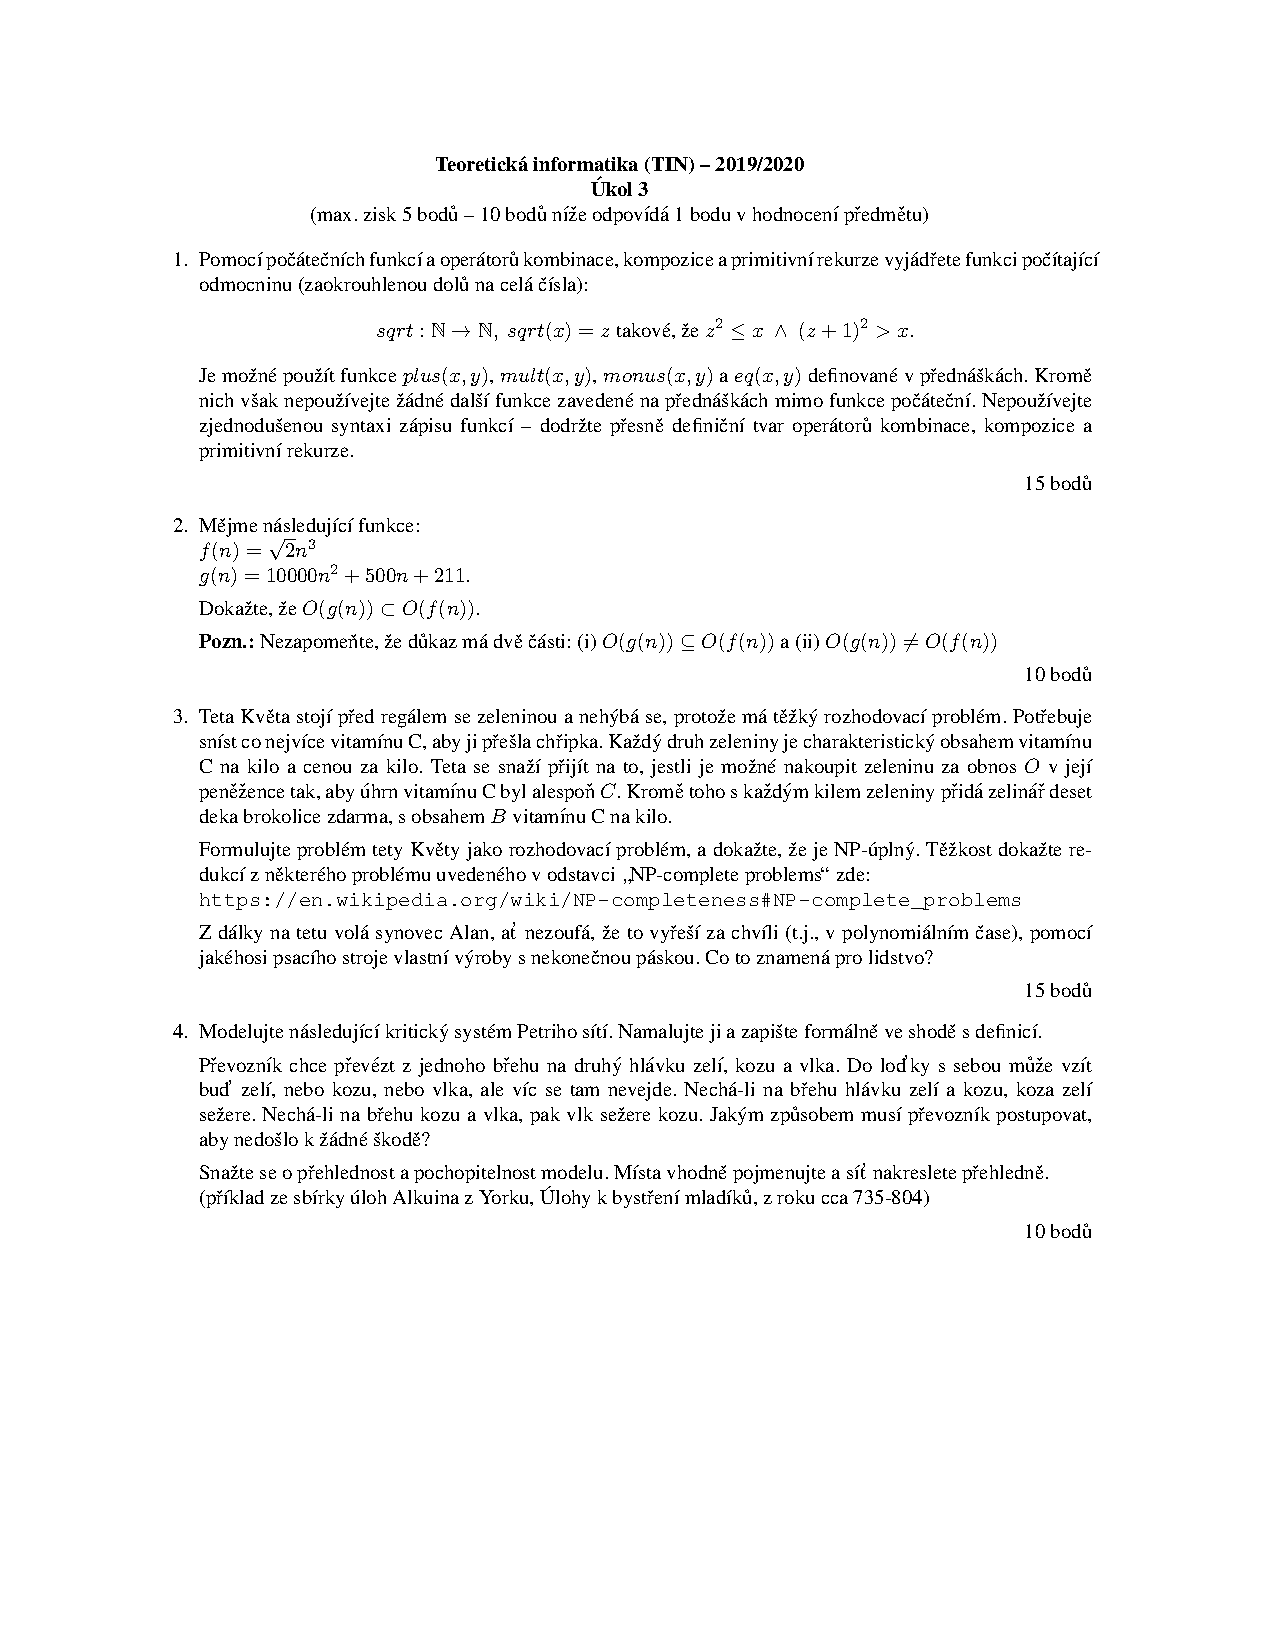
\includepdf[pagecommand={},width=1.5\textwidth]{zadanie3.pdf}

% Task 1
\section{1.úloha}
\newpage

% Task 2
\section{2.úloha}
Zostrojme si graf funkcie pre $ f(n) = \sqrt{2} n^3$ a pre $ g(n) = 10000n^2 + 500n + 211 $. \\

\begin{figure}[H]
    \centering
	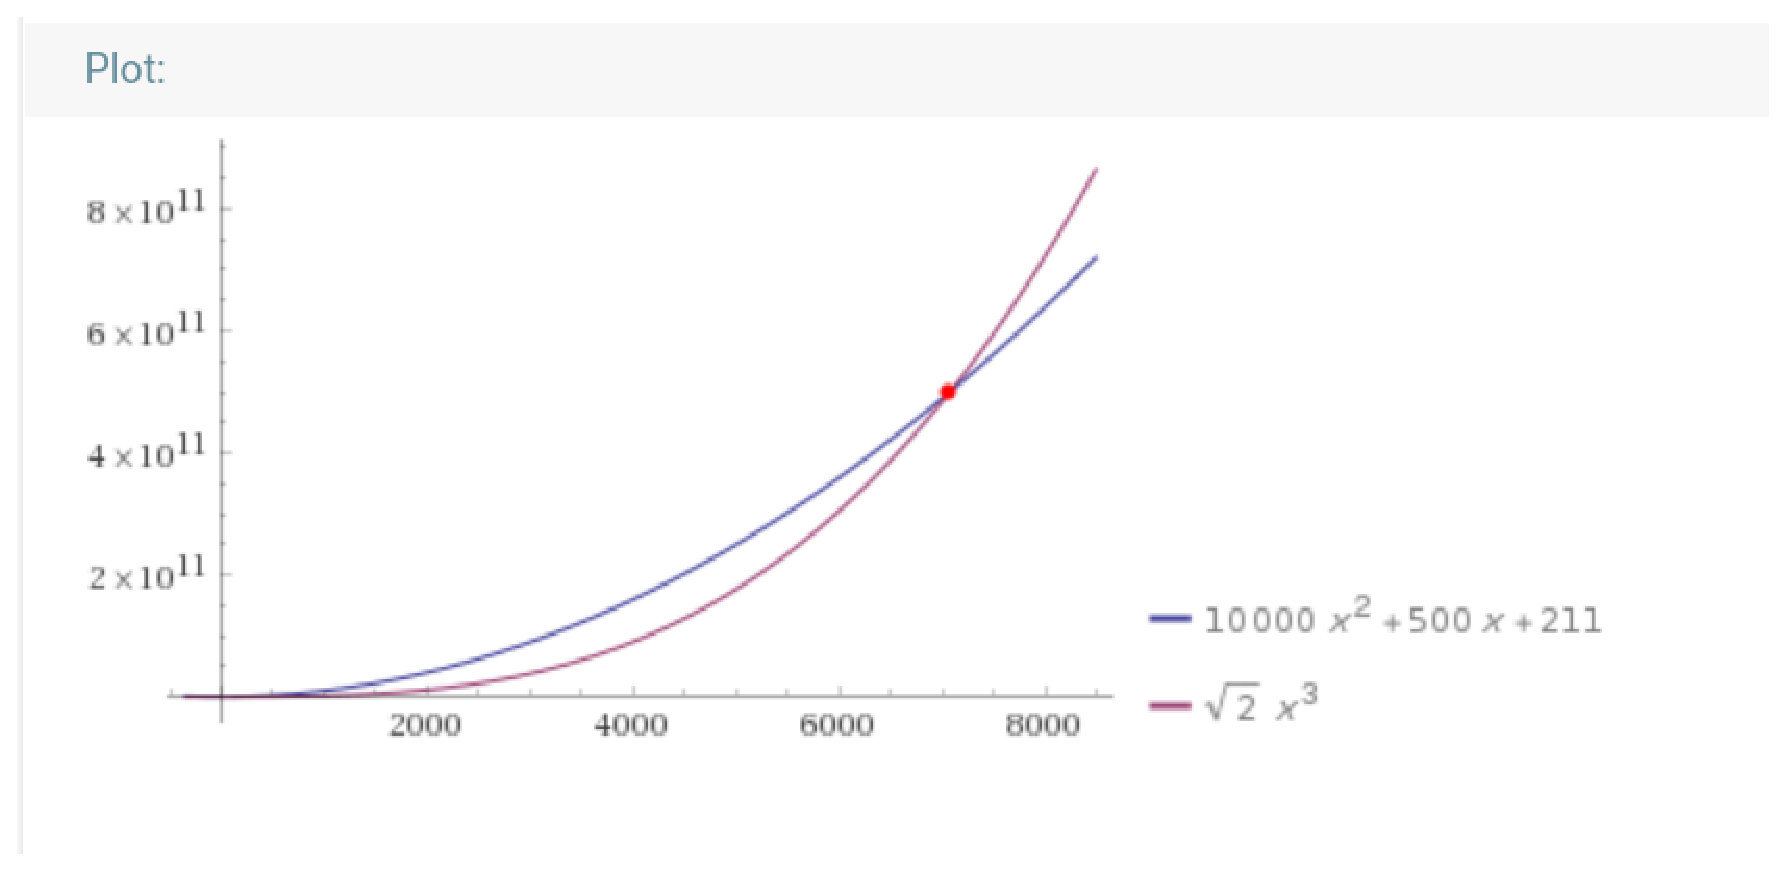
\includegraphics[width=\textwidth]{2plot.eps}
    \caption{f(x) a g(x)}
    \label{2plot}
\end{figure}


Diskriminant $D$ kubickej rovnice $ \sqrt{2}n^3 -10000n^2 -500n -211 = 0$ vypočítame podľa vzťahu: 
\begin{align*}
    D & = 18abcd -4b^3d + b^2c^2 - 4ac^3 - 27a^2d^2 \\
    D & = 18*\sqrt{2}*(-10000)*(-500)*(-211) & \\
      & -4*(-10000)^3*(-211) & \\
      & +(-10000)^2*(-500)^2 & \\ 
      & -4*\sqrt{2}*(-500)^3 & \\
      & -27*\sqrt{2}^2*(-211)^2 \\
    D &= -8.1902*10^{14}
\end{align*}

$D < 0$, rovnica má jeden reálny koreň.

Na obrázku \ref{2plot} vidíme priesečník grafov dvoch funkcí. Riešením rovnice $ f(x) = g(x) $ získame x-ové súradnice priesečníkov grafov,\footnote{Nástroj na výpocět kubickej rovnice: https://www.wolframalpha.com/widgets/view.jsp?id=3f4366aeb9c157cf9a30c90693eafc55} ich dosadením do predpisu funkcie získame y-ové súradnice.

\label{2equation}
\begin{align*}
    f(n) & = g(n) \\
   \sqrt{2} n^3 - 10000n^2 -500n -211 & = 0 \\
    n & = 7071.1
\end{align*}

\newpage
\paragraph{Dôkaz:}\mbox{{}}\\
\begin{enumerate}
    \item Z výsledkov rovnice a z grafu funkcí(Obr. \ref{2plot}) vyplíva, že od $n = 7072$ je $ f(n) > g(n)$. Obidve funkcie majú rovnaký definičný obor, teda môžeme povedať, že $ O(g(n)) \subseteq O(f(n)) $.

    \item Vieme, že výsledkom rovnice je len jeden jediný realný koreň(D < 0), a je naprosto zrejmé, že od $ n = 7072 $ sa tieto dve funkcie nikde inde nerovnajú, tak potom $ O(g(n)) \neq O(f(n)) $.
\end{enumerate}

\paragraph{Teda:}\mbox{{}}\\
$ O(g(n)) \subseteq O(f(n)) \land O(g(n)) \neq O(f(n)) \Rightarrow O(g(n)) \subset O(f(n)) $.


\newpage
% Task 3
\section{3.úloha}
\newpage

% Task 4
\section{4.úloha}
\newpage




























Test \cite{AA}







\newpage
\section{Literatura}
\bibliographystyle{czechiso}
\begin{flushleft}
    \bibliography{quotation}
    \end{flushleft}

\end{document}
